\section{Задачи RMQ и LCA}
Динамическая задача RMQ/RSQ:
дерево отрезков, оценка $\O(\log n)$
для запросов суммы/минимума
и изменения элемента.
Дерево отрезков.
Статический вариант задачи RMQ:
полное предвычисление
($\O(n^2)$ на предобработку, $\O(1)$ на запрос),
метод разреженной таблицы
($\O(n \log n)$ на предобработку, $\O(1)$ на запрос).
Задача LCA: эйлеров обход дерева,
сведение к задаче RMQ, двоичные подъёмы.
Сведение RMQ к ±1-RMQ.

\subsection{RMQ}
RMQ --- Range Minimum Query, минимальный элемент на отрезке.
RSQ --- Range Sum Query, сумма на отрезке.

Дерево отрезков, в вершинах --- индексы,
покрываемые поддеревом:

\begin{center}
    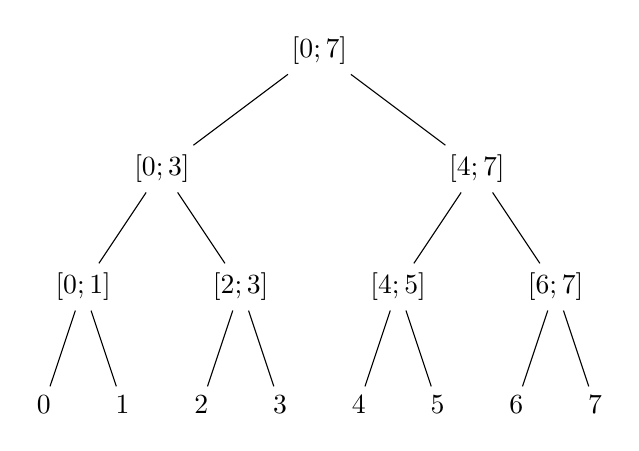
\begin{tikzpicture}
        \node { $[0; 7]$ }
            [level 1/.style={sibling distance=40mm}]
            [level 2/.style={sibling distance=20mm}]
            [level 3/.style={sibling distance=10mm}]
            child {
                node { $[0; 3]$ }
                child {
                    node { $[0; 1]$ }
                    child { node { $0$ } }
                    child { node { $1$ } }
                }
                child {
                    node { $[2; 3]$ }
                    child { node { $2$ } }
                    child { node { $3$ } }
                }
            }
            child {
                node { $[4; 7]$ }
                child {
                    node { $[4; 5]$ }
                    child { node { $4$ } }
                    child { node { $5$ } }
                }
                child {
                    node { $[6; 7]$ }
                    child { node { $6$ } }
                    child { node { $7$ } }
                }
            };
    \end{tikzpicture}
\end{center}

В каждой вершине хранится минимум в её поддереве.
Тогда обновление дерева при обновлении элемента
--- проход вверх по дереву за $\O(\log n)$.

Ответ на запрос: найти поддеревья, покрываемые
запросом целиком, и линейно составить ответ из них.
Поэтому работает не только для минимума,
а для любой ассоциативной операции.

Докажем оценку времени ответа на запрос $\O(\log n)$:
в каждом дереве запрос может либо
\begin{itemize}
    \item Покрывать дерево целиком
    --- тогда получаем ответ за $\O(1)$

    \item Полностью находиться в
    левом или правом поддереве
    --- тогда происходит один спуск

    \item Охватывать часть левого и часть правого поддерева
    --- тогда происходит два спуска,
    но это может произойти не более одного раза,
    т.к. после этого в левом поддереве
    подзапрос всегда будет касаться правой границы,
    а в правом --- левой
\end{itemize}

Поэтому для поиска максимальных по включению поддеревьев
достаточно совершить не более 2 спусков по дереву,
т.е. $\O(\log n)$ действий.

\subsubsection{Динамический вариант}
Полное предвычисление --- предподсчитаем ответы
на задачу для всех отрезков, очевидно, $\O(n^2)$.

Метод разрежённой таблицы работает только для ассоциативных
\emph{идемпотентных} операций, как минимум.
Суть: для каждого $i$ предподсчитаем $f([i; i + 2^k - 1])$:
\begin{align*}
    f([i; i]) & = a[i] \\
    f([i; i + 2^{k + 1} - 1]) & = f([i; i + 2^k - 1]) \circ f([i + 2^k; i + 2^{k + 1} - 1]) \\
\end{align*}

Тогда
\begin{align*}
    h(n) & = 2^{\floor{\log_2 n}} \\
    f([i; j]) & = f([i; i + h(j - i)]) \circ f([j - h(j - i); i]) \\
\end{align*}

Поскольку операция идемпотентна, нас не волнует пересечение
отрезков ${[i; i + h(j - i)]}$ и ${[j - h(j - i); i]}$:
\begin{center}
    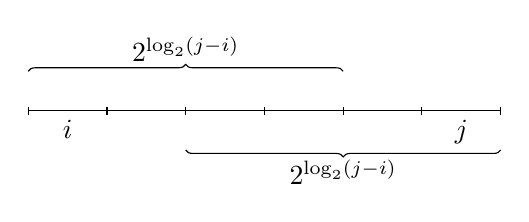
\begin{tikzpicture}
        \draw (0, 0.5) -- +(6, 0);
        \foreach \x in {0,...,6} {
            \draw (\x,0.45) -- +(0,0.1);
        }
        \draw[decorate,decoration=brace] (0,1) -- node[anchor=south] {$2^{\floor{\log_2 (j - i)}}$} +(4,0);
        \draw[decorate,decoration=brace] (6,0) -- node[anchor=north] {$2^{\floor{\log_2 (j - i)}}$} +(-4,0);
        \node[anchor=north] at (0.5, 0.5) {$i$};
        \node[anchor=north] at (5.5, 0.5) {$j$};
    \end{tikzpicture}
\end{center}

\subsection{LCA}
--- Lowest Common Ancestor.

\subsubsection{Двоичные подъёмы}
--- запишем для каждой вершины
её предка степени 0, 1, 2, 4, 8, и т.д., дальше очевидно.
Асимптотика --- $\langle \O(n \log h); \O(\log h) \rangle$,
где $h$ --- глубина дерева.

\subsection{LCA $\to$ RMQ $\pm 1$}
Можно свести к RMQ через обход дерева в глубину
(эйлеров обход графа, рёбра которого --- сдвоенные рёбра дерева):
выписать вершины в порядке входа вместе с глубинами.

\begin{center}
    \begin{tikzpicture}
        \node {1}
            child {
                node {2}
                child { node {3} }
                child { node {4} }
            }
            child {
                node {5}
                child[missing]
                child { node {6} }
            };
    \end{tikzpicture}

    \bigskip

    \begin{tabular}{r|ccccccccccc|}
        Вершина & 1 & 2 & 3 & 2 & 4 & 2 & 1 & 5 & 6 & 5 & 1 \\
        Глубина & 0 & 1 & 2 & 1 & 2 & 1 & 0 & 1 & 2 & 1 & 0 \\
    \end{tabular}
\end{center}

Можно заметить, что с момента, когда мы зашли в поддерево,
до момента, когда мы из него вышли, корень этого поддерева
--- самая верхняя вершина.
Тогда между первыми попаданиями в вершины $u$ и $v$
самая верхняя вершина, в которой мы можем оказаться
--- их наименьший общий предок.
Тогда RMQ по глубине в выписанном массиве между этими попаданиями
даст нам искомую вершину.

Получили $\langle \O(n); \O(1) \rangle$-\emph{сведение}
(т.е. преобразование работает за это время, не сам алгоритм)
LCA к RMQ.

\subsection{RMQ $\to$ LCA}
Построим декартово дерево по неявному ключу.
Тогда в нём RMQ на отрезке --- LCA вершин,
соответствующих границам этого отрезка:

\begin{center}
    \begin{tabular}{r|ccccccccc|}
        Массив & 17 & 0 & 36 & 16 & 23 & 15 & 42 & 18 & 20 \\
    \end{tabular}

    \begin{tikzpicture}
        \node {0}
            [level 1/.style={sibling distance=60mm}]
            [level 2/.style={sibling distance=30mm}]
            [level 3/.style={sibling distance=15mm}]
            child { node {17} }
            child {
                node {15}
                child {
                    node {16}
                    child { node {36} }
                    child { node {23} }
                }
                child {
                    node {18}
                    child { node {42} }
                    child { node {20} }
                }
            };
    \end{tikzpicture}
\end{center}

Если $v_k = LCA(v_i; v_j)$, то
$v_i$ и $v_j$ лежат в разных поддеревьях $v_k$,
следовательно, $i \le k \le j$.
Поэтому поддерево $v_k$ содержит вершины $v_i, \ldots, v_j$
и $x(v_k)$ из них минимально, поэтому
$x(LCA(v_i; v_j)) = RMQ(i; j)$.

Декартово дерево по неявному ключу строится за $\O(n)$,
запрос сводится за $\O(1)$,
поэтому получили $\langle \O(n); \O(1) \rangle$-сведение
RMQ к LCA.

\subsection{Алгоритм Фарака-Колтона и Бендера}
$\text{RMQ}\pm 1$ (где соседние элементы отличаются
либо на $1$, либо на $-1$, никогда не на $0$ или любое другое число)
можно решить за $\langle \O(n); \O(1) \rangle$:
разобьём массив на блоки по $k = \frac{1}{2} \log_2 n$,
для каждого блока посчитаем его минимум, на блоках
применим разрежённую таблицу.
Построение разрежённой таблицы:
\begin{gather*}
    \frac{n}{k} \log \frac{n}{k} = \\
    = \frac{2n}{\log_2 n} \log \parens{\frac{2n}{\log_2 n}} = \\
    = \frac{2n}{\log_2 n} \parens{1 + \log_2 n - \log_2 \log_2 n} = \\
    = \frac{2n}{\log_2 n} + 2n - 2n \frac{\log_2 \log_2 n}{\log_2 n} \le \\
    \le \frac{2n}{\log_2 n} + 2n \in \O(n)
\end{gather*}

Запрос $RMQ[l; r]$ разбивается на части
--- от $l$ до конца блока, от начала блока до $r$
и между блоками (последний --- за $\O(1)$).
Хотим запросы внутри блока также делать за $\O(1)$.

Разности соседних элементов --- всегда $\pm 1$.
Тогда существует $2^{k - 1}$ различных наборов разностей
внутри блока.
\[ 2^{k - 1} = 2^{\frac{1}{2} \log_2 n - 1} = \frac{\sqrt{n}}{2} \in \O(\sqrt{n}) \]

Предподсчитаем ответы также для $\O(\sqrt{n})$
различных блоков, и для каждого блока разбиения предподсчитаем
его тип (например, индекс в массиве записывается
как разности соседних элементов, где $1$ записывается
единичным битом, а $-1$ --- нулевым).
Поскольку $k = \frac{1}{2} \log_2 n$,
то $2^{k - 1} < n$ всегда поместится в машинное слово.

Табличное значение одного блока можно посчитать
за $k^2 = \parens{\log_2 n}^2 = \O(\log^2 n)$.
Все табличные значения вместе
--- за $\O(\sqrt{n} \cdot \log^2 n) \subset \O(n)$.

Таким образом, все предподсчёты вместе занимают $\O(n)$
времени, а запрос выполняется за $\O(1)$.

При этом мы также получили
$\langle \O(n); \O(1) \rangle$-сведения
RMQ $\to$ LCA и LCA $\to$ RMQ $\pm 1$,
что означает, что каждая из этих задач решается за
$\langle \O(n); \O(1) \rangle$.
